\section{Outreach}
\label{sec:outreach}
Conveying additional useful information about the results of
a generic ``signature-based'' search such as the one described
in this note is a difficult issue.  
Here we attempt to present our result in the most general 
way.

Models of new physics in the dilepton final state 
can be confronted in an approximate way by simple 
generator-level studies that 
compare the expected number of events in \lumi\
with our upper limits in Sec.~\ref{sec:limits}.  The key ingredients
of such studies are the kinematical cuts described 
in this note, the lepton efficiencies, and the detector
responses for \Ht, $y$, and \met.

The muon identification efficiency is $\approx 96\%$;
the electron identification efficiency varies approximately linearly from $\approx$ 60\% at 
\pt = 10 GeV to 90\% for \pt $>$ 30 GeV.  
%
The lepton isolation efficiency depends on the lepton momentum, as well as on the jet activity in the 
event.
In $t\bar{t}$ events, it varies approximately linearly from $\approx 73\%$ (muons)
and $\approx 82\%$ (electrons) at \pt = 10 GeV to $\approx 97\%$ for \pt $>$ 60 GeV. 
In LM1 (LM3,LM6) events, this efficiency is decreased by $\approx$5--10\% ($\approx$10\%,$\approx$5\%)over the whole momentum spectrum.
%
The average detector responses (the reconstructed quantity divided by the generated quantity) 
for \Ht, $y$ and \met\ are consistent with 1 within the 5\% jet energy scale uncertainty.
The experimental resolutions on these quantities are 9\%, 12\% and 12\%, respectively.

To justify the statements in the previous paragraph 
about the detector responses, we plot 
in Figure~\ref{fig:response} the average response for 
\Ht, $y$ and \met, as well as the
efficiency for the cuts on these quantities used in defining the
signal region.

The lepton identification and isolation efficiencies are displayed for the dominant
\ttbar\ background in Fig.~\ref{fig:leptoneff}. The isolation efficiencies for the LM1
and LM3 processes are displayed in Fig.~\ref{fig:leptoniso}, which shows the decrease
in isolation efficiency resulting from the large hadronic activity in these events.


%Using this information as well as the kinematical
%cuts described in Section~\ref{sec:eventSel} and the lepton efficiencies
%of Figures~\ref{fig:effttbar}, one should be able to confront
%any existing or future model via a relatively simple generator 
%level study by comparing the expected number of events in 35 pb$^{-1}$
%with our upper limit of 4.1 events.

\begin{figure}[tbh]
\begin{center}
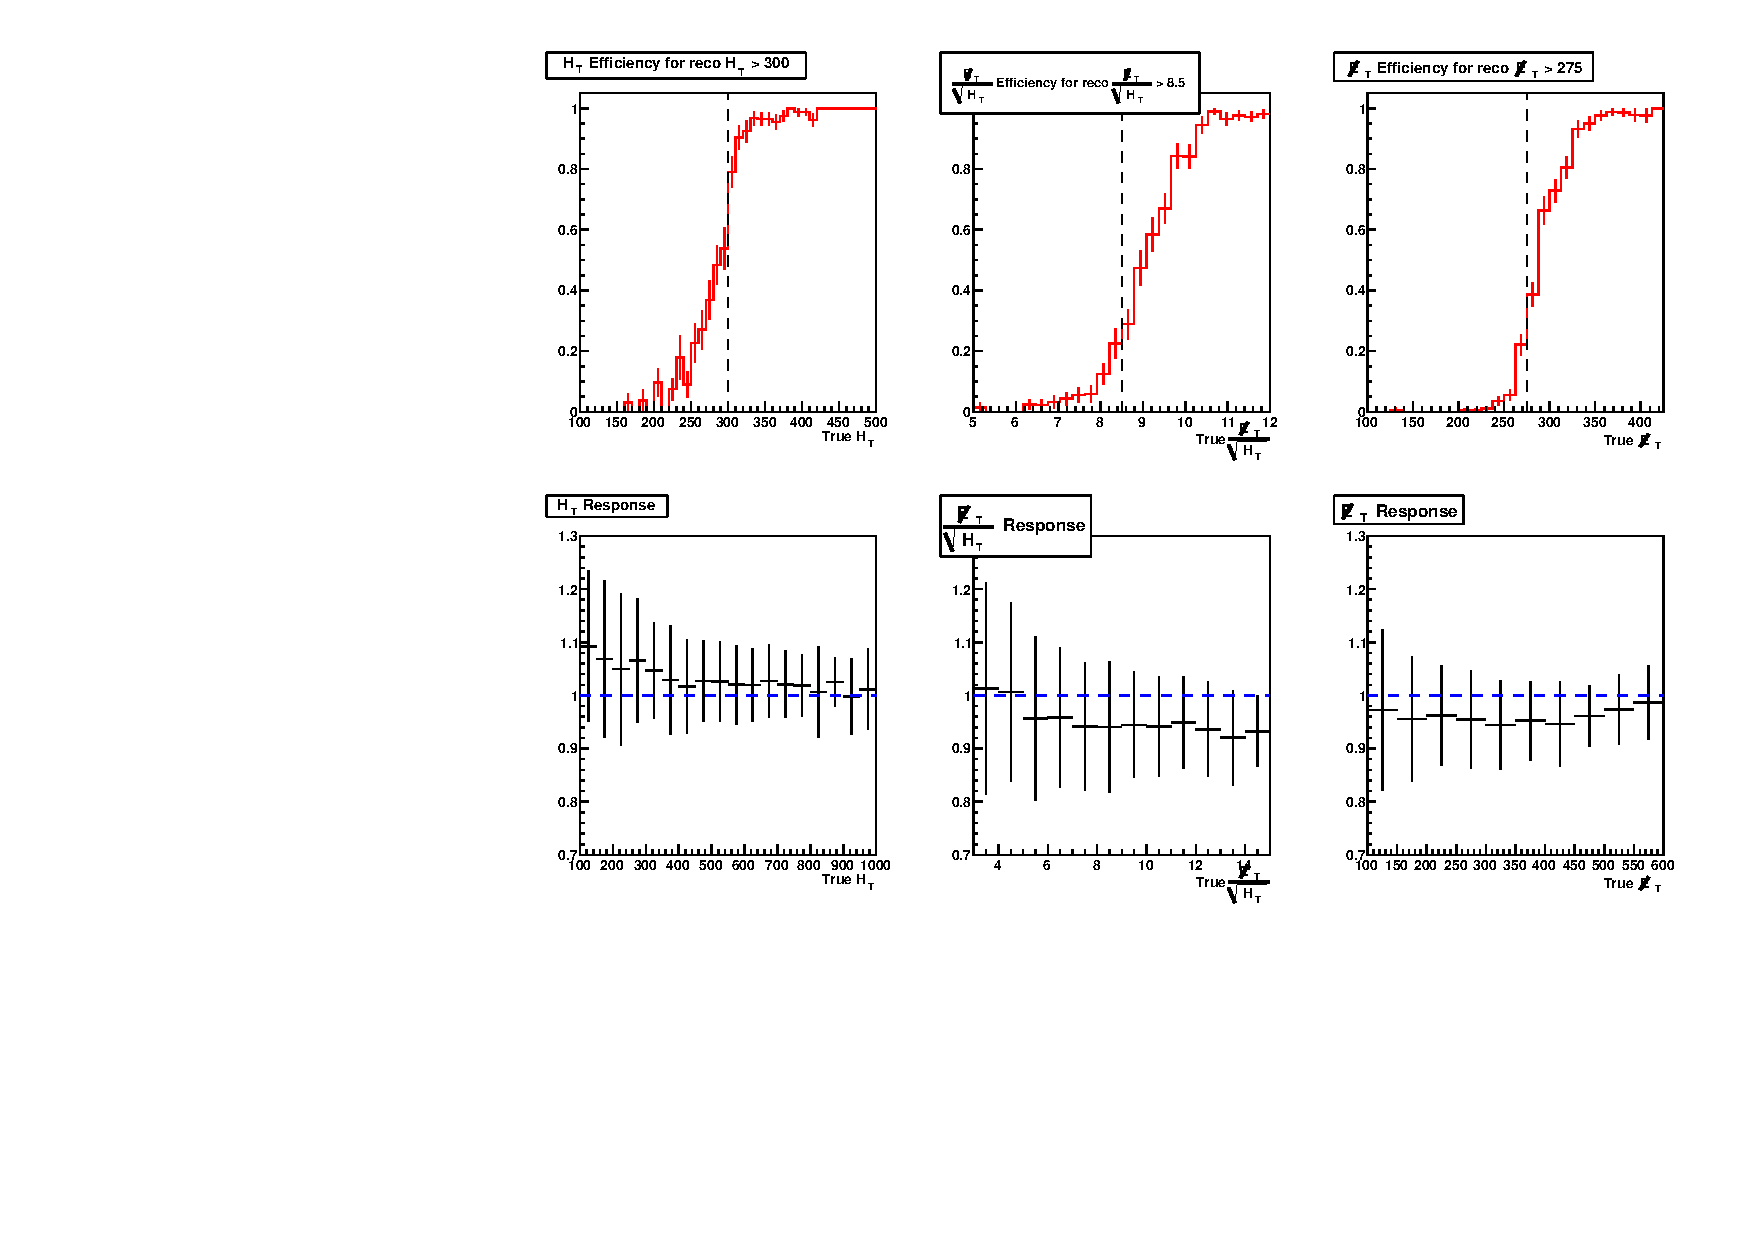
\includegraphics[width=\linewidth]{plots/lm1_SelectionEfficiency.pdf}
\caption{\label{fig:response} 
Top plots: the efficiencies to pass the signal region requirements (vertical dashed lines) on \Ht\ (left), $y$ (middle) and \met\ (right) as a function
of the generated quantities. Bottom plots: the average detector responses for \Ht, $y$ and \met\ and the corresponding RMS (error bars), as a function 
of the generated quantities. The response is defined as the ratio of the reconstructed quantity
to the true quantity in MC.  These plots are done using the LM1
Monte Carlo, but they are not expected to depend strongly on 
the underlying physics.
}
\end{center}
\end{figure}

\begin{figure}[tbh]
\begin{center}
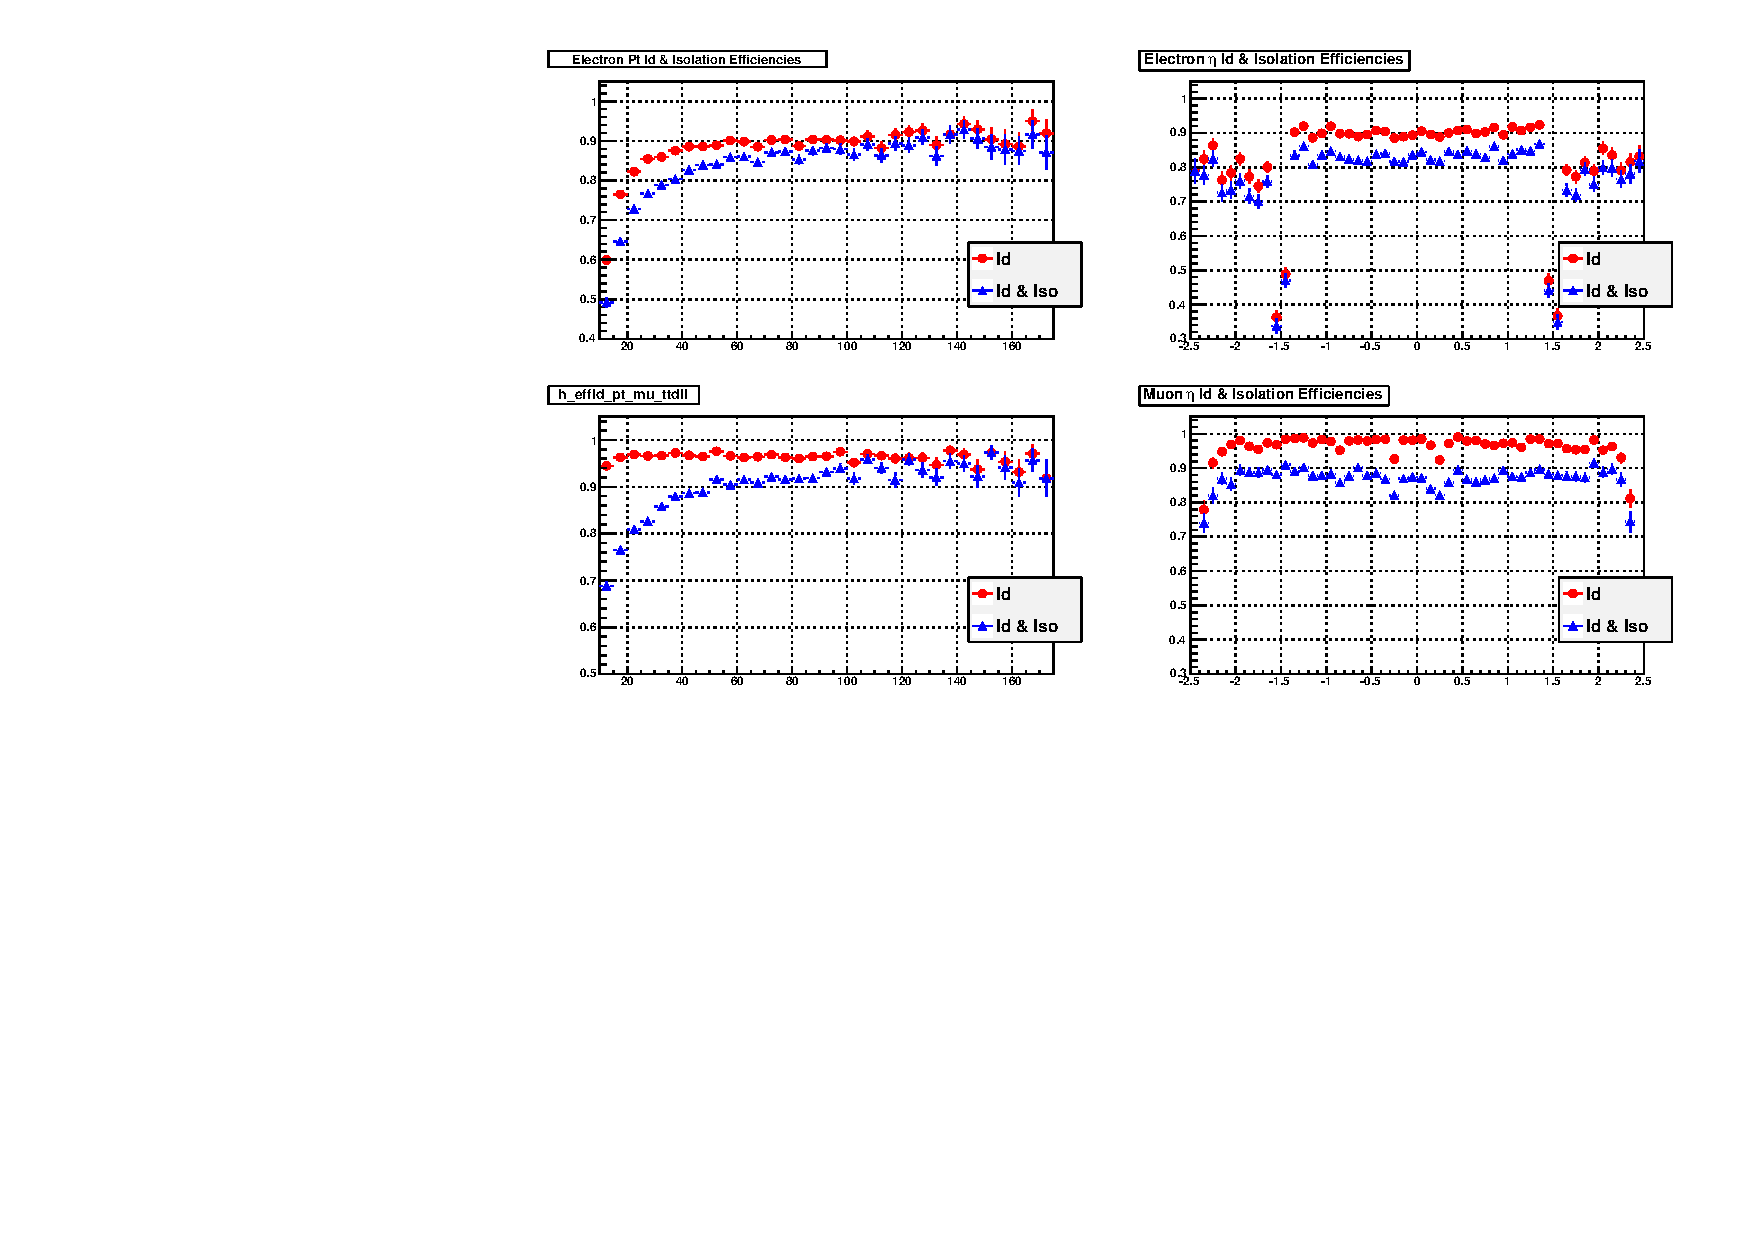
\includegraphics[width=\linewidth]{plots/ttdil_leptonEfficiencies.pdf}
\caption{\label{fig:leptoneff} 
The lepton identification and isolation efficiencies in \ttbar\ MC for electrons (top) and muons (bottom)
vs. \pt\ (left) and $\eta$ (right).
}
\end{center}
\end{figure}

\begin{figure}[tbh]
\begin{center}
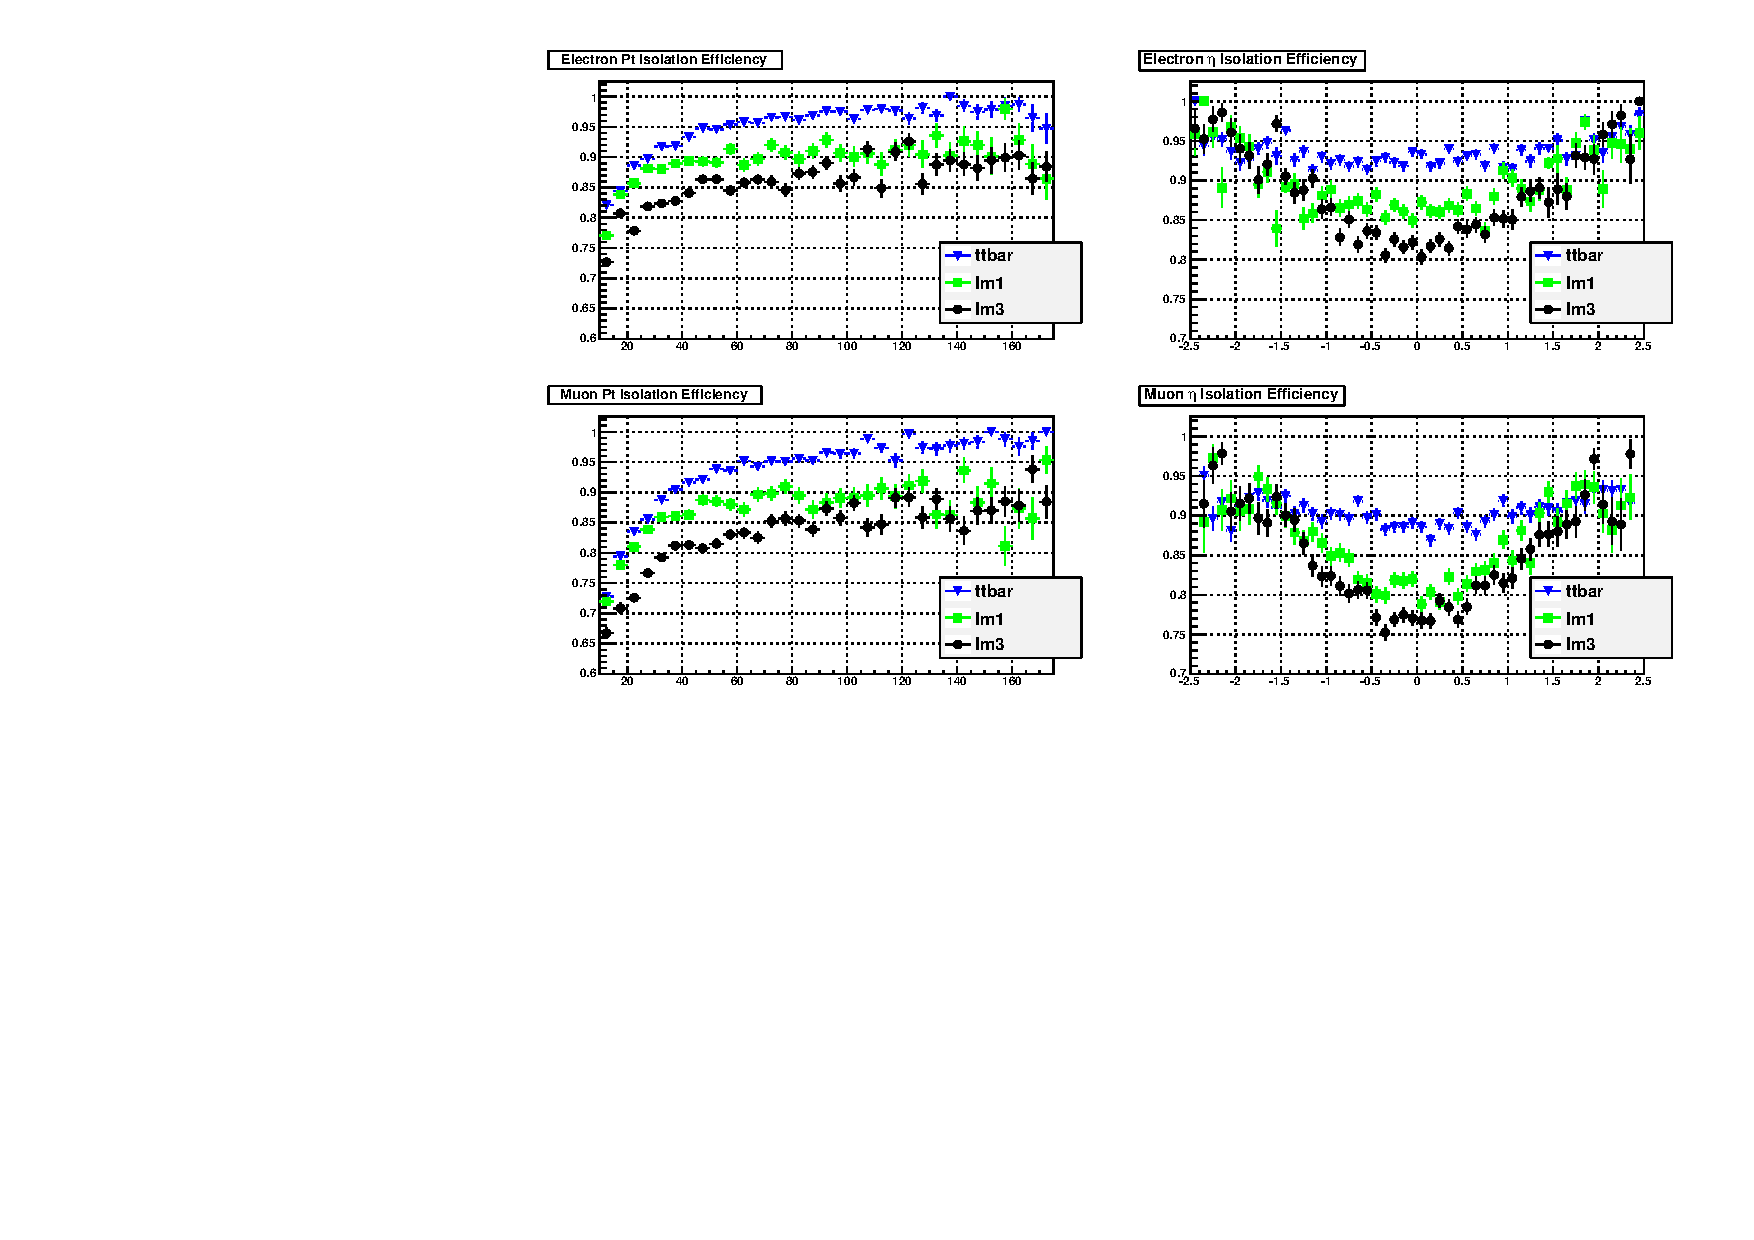
\includegraphics[width=\linewidth]{plots/tt_and_lm_isolationEfficiencies.pdf}
\caption{\label{fig:leptoniso} 
The lepton isolation efficiencies for \ttbar, LM1 and LM3 MC for electrons (top) and muons (bottom)
vs. \pt\ (left) and $\eta$ (right).
}
\end{center}
\end{figure}
